
\section{Driver}
\label{sec:driver}

The part that does all the acting in this world is the drivers. A
driver looks at the world (\ref{sec:sight}), assesses the situation
and reacts accordingly (\ref{sec:animus}), decides about which
way to go (\ref{sec:driverJunctions}) and eventually steers the
vehicle (\ref{sec:driverInfluence}). Drivers have a character
(\ref{sec:character}), physical conditions (\ref{sec:physics}) and could
even take drugs (\ref{sec:drugs}). \\

\subsection{Animus}
\label{sec:animus}

The Animus is the brain of the driver. Here all waypoints 
(\ref{sec:wayPointSystem}) are processed and decisions are made. \\

\noindent The Animus only knows the current speed limit on the lane 
(before the driver has seen any speed limit signs this is some global
default value). It then assesses the situation in following order:

\begin{itemize}
\item Look at the world and collect way points (assessment)
\item Process them and let them act on the acceleration and deceleration activators
\item Do the way point specific stuff (e.g. remember speed limit)
\item Calculate the resulting acceleration value
\end{itemize}

\subsubsection{Assessment and decision making}
\label{sec:assessment}

Based on the way points the driver has to decide whether to accelerate or
decelerate or keep the current speed. Since he can see several way points
at once, we developed a system where all the way points have a certain effect 
on that decision. Figure \ref{fig:animus} shows this process.

\begin{figure}[H]
\begin{center}
\includegraphics[width=10cm]{images/animus.png}
\end{center}
\caption{How the waypoints influence the acceleration}
\label{fig:animus}
\end{figure}

The influences on the acceleration and deceleration are weighted, so for 
instance the vehicle way points have a higher weight so it influences the 
deceleration more than a speed way point can influence the acceleration.
The acceleration and deceleration in this picture are values ranging from
0 to 1. After all way points had their influence, the two values are then
subtracted. The difference is then the effective acceleration value that 
goes to the vehicle; -1 is full braking and 1 is full acceleration which
both depend on the vehicles properties. \\

With this system the driver always drives as fast as he is allowed to
as long as there is nothing else interrupting his way.


\subsubsection{The estimation of another vehicle's speed}

To know whether another vehicle is approaching (because it moves 
more slowly) or not, we could have just implemented a method on the
way point that returns the speed of it's vehicle to the driver that
is assessing. But we wanted it to be more realistic, the drivers should have
to estimate the speed of the other traffic participants. They can
therefore only retrieve the somewhat fuzzy distance (\ref{sec:movingWPDistance})
to the other waypoints. A driver then has to remember the distance
of the nearest vehicle, until the next assessment cycle. It can then
compare the remembered distance with the new one and knows, whether the
vehicle is approaching or not and how fast.

\subsubsection{Following another vehicle}

The driver always tries to keep a certain security distance to the
vehicle in front of him, which is twice the speed that he is going (e.g. $ 50 km/h => 100m$).
When the distance of the vehicle in front falls below that value, the
animus begins to influence the deceleration value (\ref{sec:assessment}).
The nearer the vehicle is, the higher is the influence.

\subsubsection{Decisions in junctions}

The behaviour in junctions is a bit extended. As described in 
\ref{sec:junctionWPfinding}, the way point finding is a bit more intelligent
to regard the right of way. Once they are found, the process is the same
though.

\subsection{Physics}
\label{sec:physics}

The physics objects define the physical conditions of the driver. Every
driver has one of these objects. They provide the following properties:

\begin{itemize}
\item \textbf{The sight} How far the driver can see
\item \textbf{The field of view (angle)} The opening of the driver view
\item \textbf{Update interval} The interval of the assessment cycles
\item \textbf{Drugs}
\end{itemize}

\subsubsection{Drugs}
\label{sec:drugs}

Drugs are objects than can influence the properties mentioned above in the
physics section. They are merely just implemented and prepared but not 
in use yet.

\subsection{Character}
\label{sec:character}

The drivers are prepared to have some sort of character. This character
contains values like ''riskyness`` and temperament. A driver with a
high temperament accelerates faster than a Sunday driver.

\subsection{Sight}
\label{sec:sight}

At this point of process the driver only sees things ahead of him on the
lane. There are no mirrors, and it is not possible to look behind, hence
he is not able to reverse.\\

\noindent What the driver can see is limited to a field of view formed like 
a ''Pacman``. We implemented that as the \emph{driver view}, more on that in 
section \ref{sec:driverView}.

\subsection{Junctions}
\label{sec:driverJunctions}

When a driver approaches a junction, he receives the according way point
from the way point system. He then makes a decision in which direction he
wants to drive on. Since we don't have any path finding and the cars are
just driving around, this decision is randomly taken. Once decided, a
driver event is created and processed immediately which then triggers
the junction routine of the vehicle (\ref{sec:laneChanges}).

